\chapter{Ergebnisse der Klassifikation}\label{chap:Ergebnisse-der-Klassifikation}
Dieses Kapitel vergleicht die Klassifikationsergebnisse der vier Modellfamilien. Zuerst werden Accuracy und Macro-F1 gegenübergestellt. Danach zeigen die Konfusionsmatrizen, bei welchen Sorten die Modelle Fehler machen und ob sich ähnliche Verwechslungen über mehrere Modelle hinweg wiederholen.


\section{Modellvergleich}
Tabelle~\ref{tab:modelle_ergebnisse} zeigt die Ergebnisse der vier Modelle im gewählten Testsetup. Alle Modelle erreichen eine Accuracy von mindestens 0{,}917 und einen Macro-F1-Score von mindestens 0{,}929. Die Unterschiede sind klein. Das MLP erzielt mit 0{,}923 Accuracy und 0{,}934 Macro-F1 die höchsten Werte, liegt aber nur knapp vor HistGradientBoosting und der logistischen Regression.
Die geringen Abstände sprechen dagegen, das MLP als klar überlegenes Modell zu verstehen. Im Folgenden wird es als bestes Modell dieses konkreten Testlaufs betrachtet.
\begin{table}[htbp]
\centering
\begin{tabular}{lrr}
\toprule
Modell & Accuracy & Macro-F1 \\
\midrule
MLP Neural Network & 0.923 & 0.934 \\
HistGradientBoosting & 0.920 & 0.932 \\
Logistic Regression & 0.917 & 0.931 \\
Random Forest & 0.917 & 0.929 \\
\bottomrule
\end{tabular}
\caption{Vergleich der Klassifikationsmodelle im Testsetup}
\label{tab:modelle_ergebnisse}
\end{table}

\section{Einordnung der Metriken}
Die Accuracy-Werte liegen sehr nah beieinander. Zwischen dem besten und dem schwächsten Modell liegen 0{,}006 Punkte. Beim Macro-F1-Score beträgt der Abstand 0{,}005 Punkte. Die Leistungsunterschiede zwischen den Modellfamilien sind in diesem Testlauf also gering.

Der Macro-F1-Score ergänzt die Accuracy, weil er die F1-Werte der einzelnen Klassen ungewichtet mittelt \cite{scikitLearnF1Score}. Dadurch erhält jede Klasse denselben Einfluss auf die Kennzahl, unabhängig davon, wie häufig sie im Datensatz vorkommt. Für eine genauere Einordnung reichen diese beiden Kennzahlen aber nicht aus.

Abbildung~\ref{fig:Konfusionsmatrizen_Alle_Modelle} zeigt deshalb die Konfusionsmatrizen der vier untersuchten Modelle. Die Diagonale enthält die korrekt klassifizierten Bohnen, alle Werte außerhalb der Diagonale zeigen Verwechslungen zwischen Sorten.

Die Fehler verteilen sich nicht gleichmäßig über alle Klassen. \texttt{BOMBAY} wird in drei Modellen vollständig richtig erkannt; beim HistGradientBoosting liegt nur eine Beobachtung außerhalb der Diagonale. Die meisten Verwechslungen treten zwischen \texttt{DERMASON} und \texttt{SIRA} auf. Je nach Modell werden zwischen 38 und 61 Bohnen von \texttt{DERMASON} als \texttt{SIRA} klassifiziert oder umgekehrt. Ein zweites, kleineres Fehlermuster liegt zwischen \texttt{BARBUNYA} und \texttt{CALI}. Diese Struktur erscheint bei allen vier Modellen und spricht dafür, dass die betroffenen Sorten mit den verwendeten acht Merkmalen schwerer zu trennen sind als \texttt{BOMBAY}, \texttt{HOROZ} oder \texttt{SEKER}.

Damit ergänzen die Konfusionsmatrizen den Modellvergleich um die konkrete Fehlerstruktur. Die ähnlichen Muster passen auch zu den nah beieinanderliegenden Werten aus Tabelle~\ref{tab:modelle_ergebnisse}: Kein Modell löst die schwierigen Klassenverwechslungen grundsätzlich anders als die übrigen Modelle.

\begin{figure}[htbp]
  \centering
  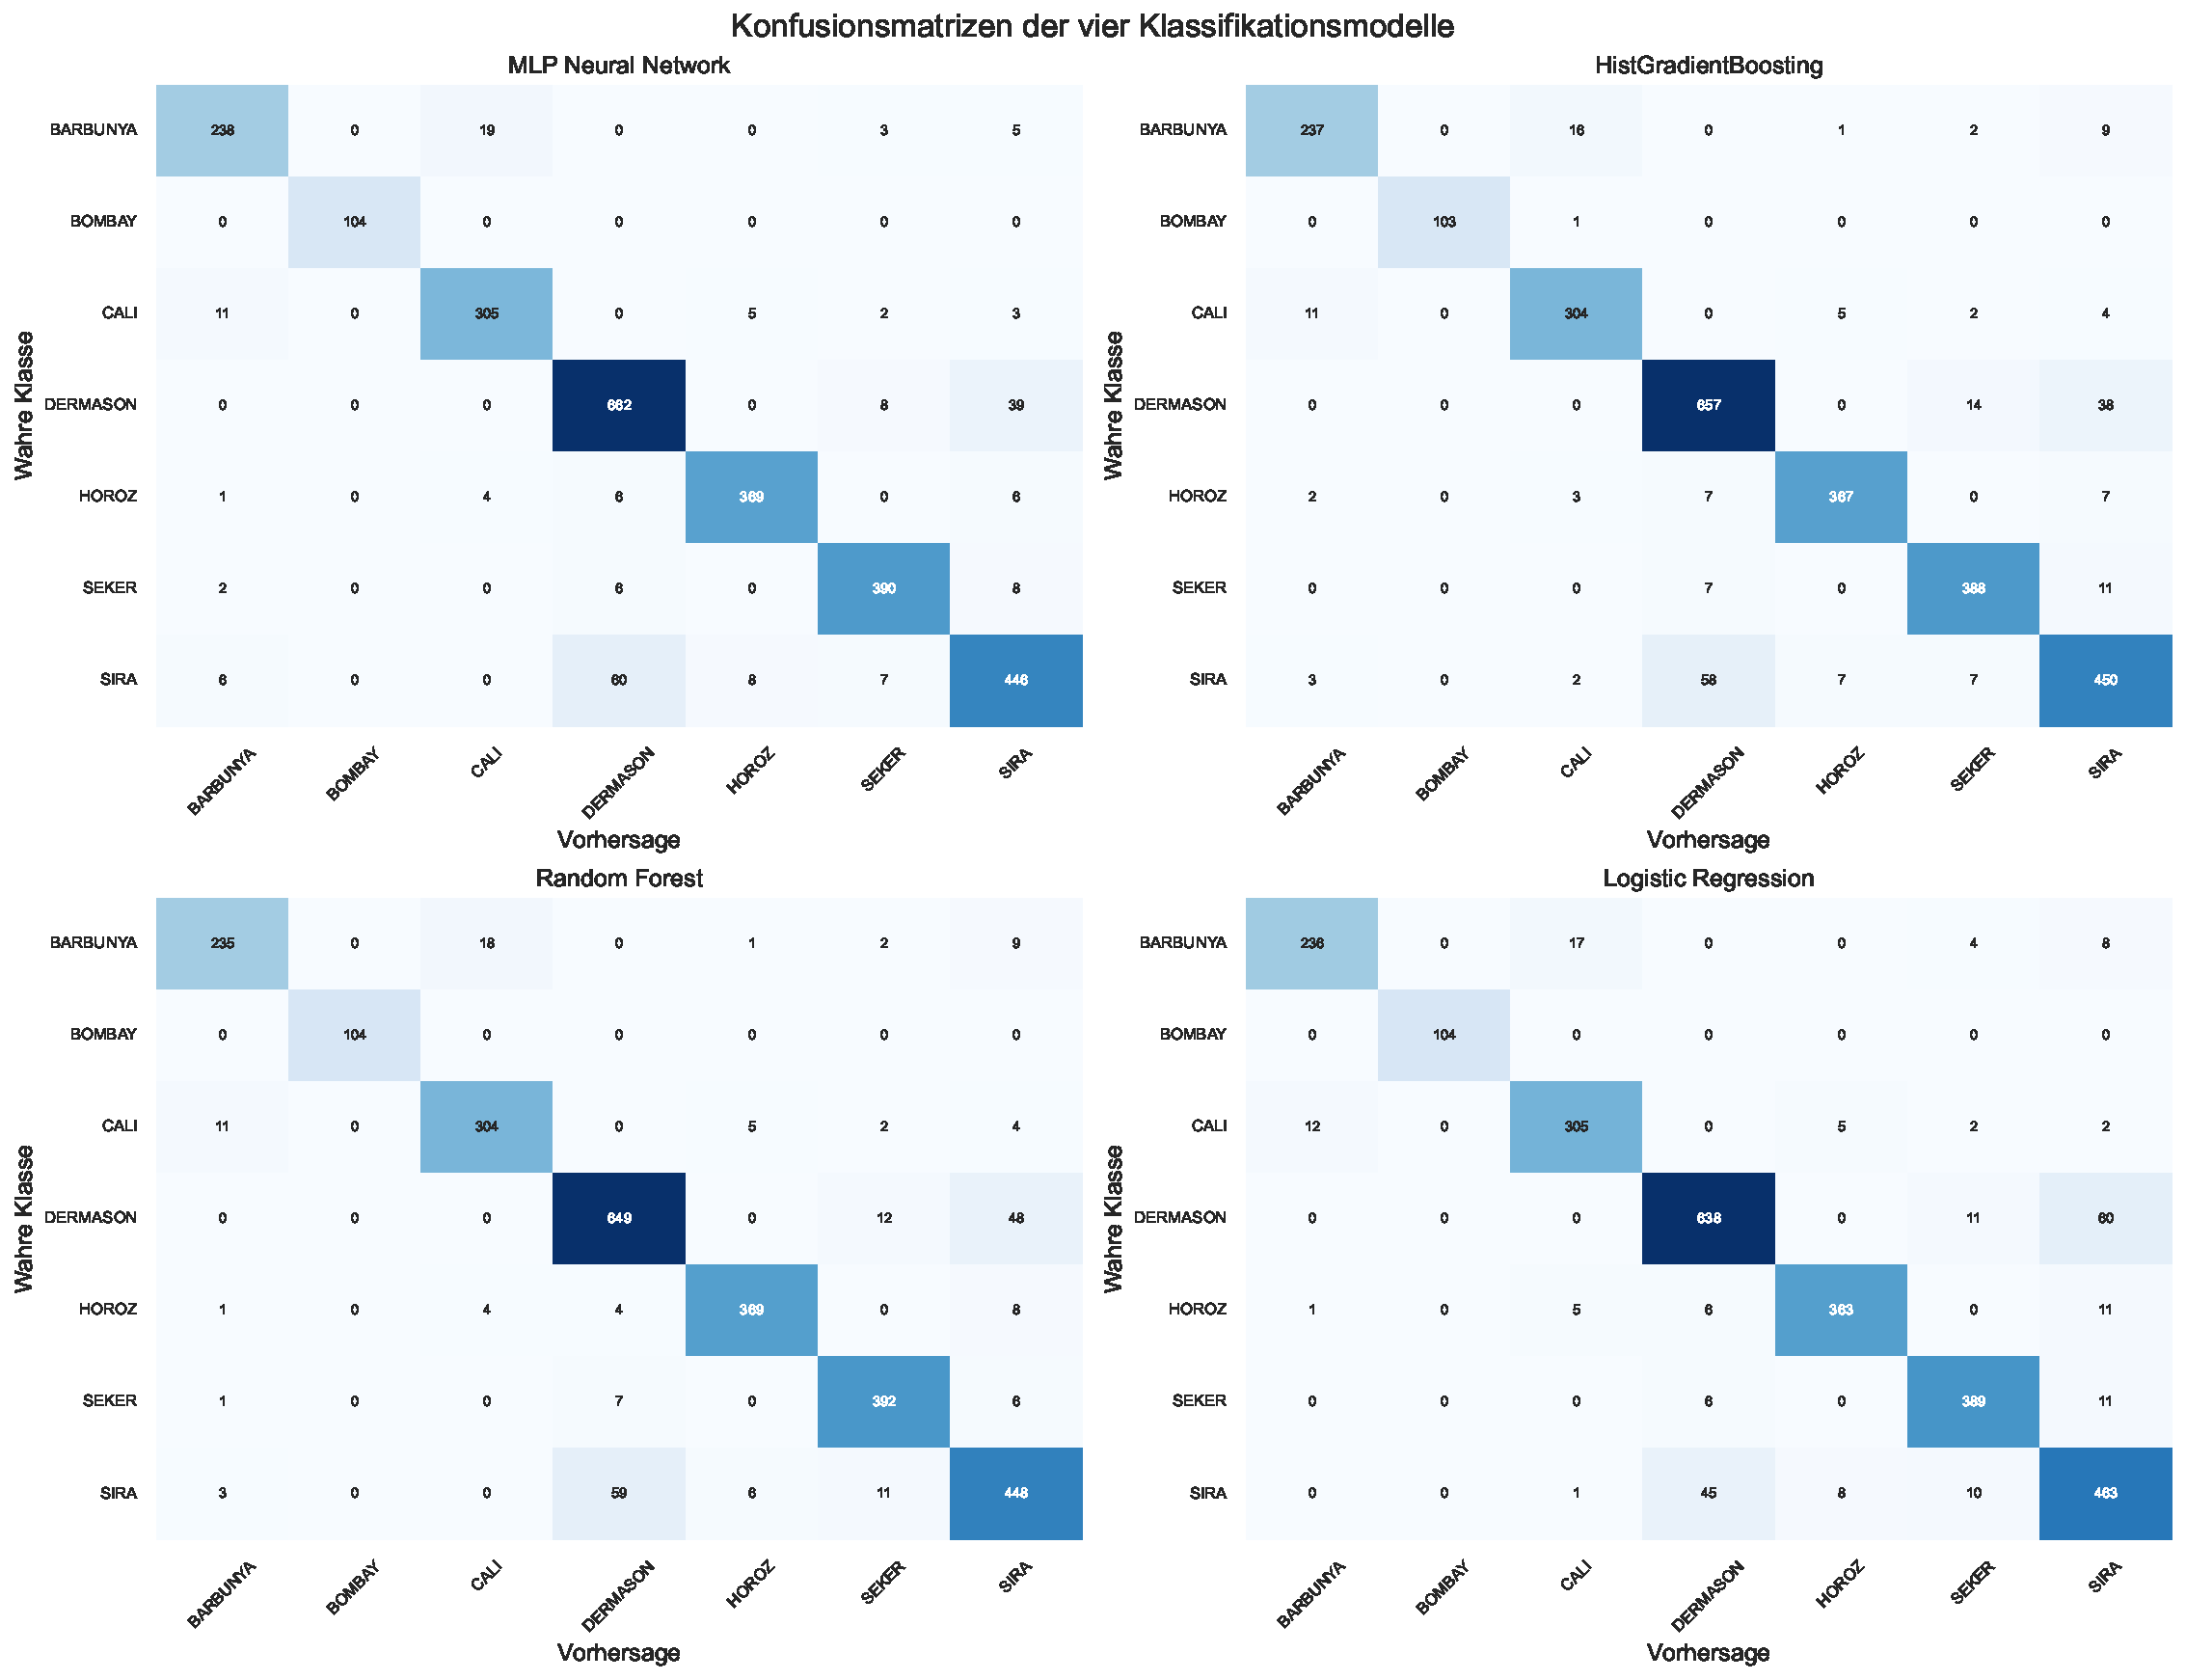
\includegraphics[width=\textwidth]{Graphics/Konfusionsmatrizen_Alle_Modelle.pdf}
  \caption{Konfusionsmatrizen der vier Klassifikationsmodelle}
  \label{fig:Konfusionsmatrizen_Alle_Modelle}
\end{figure}

\section{Zwischenfazit}

Die vier untersuchten Modelle erreichen auf dem reduzierten Feature-Set ähnliche Ergebnisse. Das MLP liegt im Testsetup knapp vorn, HistGradientBoosting folgt direkt dahinter. Die logistische Regression bleibt wegen ihrer einfacheren Struktur ein wichtiger Vergleichspunkt. Die Konfusionsmatrizen ergänzen diesen Vergleich, weil sie die Fehlerstruktur der Modelle sichtbar machen. Ob die Vorhersagen auf nachvollziehbaren Größen- und Formmerkmalen beruhen, wird im nächsten Kapitel mit XAI-Methoden untersucht.
